\chapter[Decaimiento del falso vacío en la TCC]{Decaimiento del falso vacío en la Teoría Cuántica de Campos}

%\section{Soluciones a la ecuación de movimiento}

\section{Tasa de decaimiento del falso vacío en la Teoría Cuántica de Campos}

\section{Bounces en la Teoría Cuántica de Campos}

%Habiendo desarrollado el formalismo 
Si bien al momento de calcular la tasa de decaimiento del falso vacío en la Teoría Cuántica de Campos del campo escalar haremos uso del formalismo desarrollado en el capítulo anterior adaptado, %mediante analogía con lo estudiado 
previamente debemos plantear el problema clásico correspondiente con sus respectivas condiciones de frontera y encontrar las soluciones a la ecuación de movimiento.  

Consideremos el campo escalar $\phi\qty(x)$ cuya acción $S\qty[\phi\qty(x)]$ está dada por %\footnote{$x=\qty(t, x, y, z)$ es el cuadrivector posición.} 
\begin{equation} \label{eq:accion_qft}
S\qty[\phi\qty(x)] = \int \dd[4]{x} \qty[\frac{1}{2}\qty(\pdv{\phi}{t})^2 - \frac{1}{2}\qty(\grad{\phi})^2 - U\qty(\phi) ].
\end{equation}
La densidad de potencial $U\qty(\phi)$ está dado en la figura \ref{fig:potencial_qft} 
%\footnote{$U\qty(\phi)$ es en realidad la densidad de potencial pero por conveniencia lo llamaremos simplemente potencial al no haber confusión entre ambos términos.}
. Cuenta con dos mínimos $\phi_-$ y $\phi_+$, de los cuales este último es un falso vacío por lo que, al igual que en la Mecánica Cuántica, 
%revisar terminos: "se encuentre" o "tenga una configuracion"
esperamos que, si el campo se encuentra inicialmente en $\phi_+$, 
exista una cierta probabilidad de que
pueda decaer a $\phi_-$ por tunelamiento. Resulta conveniente añadirle una constante 
%a $U\qty(\phi)$ 
de tal manera que $U\qty(\phi_+) = 0$ y la energía del falso vacío sea finita \cite{andreassen2017precision} 
\begin{figure}[b]
	\centering
	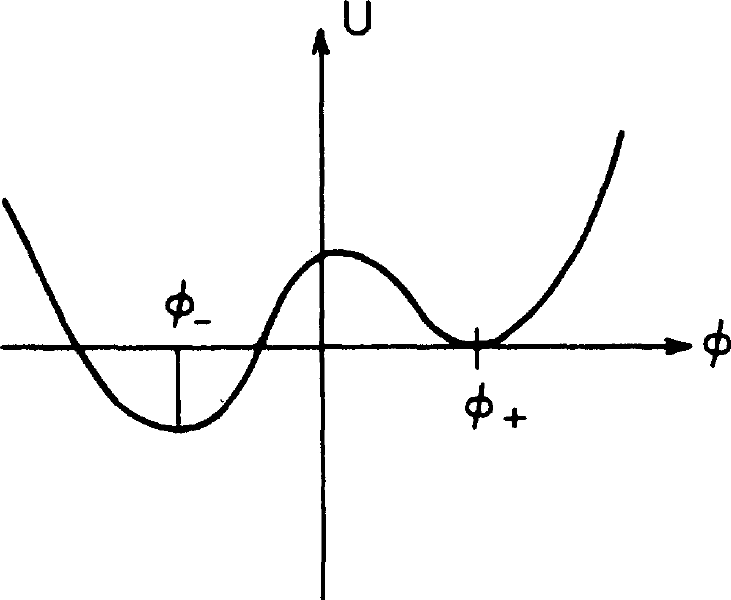
\includegraphics[scale=0.25]{FIGURAS/potencial_qft}
	\caption{Potencial en el que se encuentra el campo escalar dado por la acción \eqref{eq:accion_qft}. Notamos que cuenta con un falso vacío en $\phi_+$ \cite{callan1977fate}.}
	\label{fig:potencial_qft}
\end{figure}

Aplicando el cambio de variable \eqref{eq:tiempo_im} en la acción \eqref{eq:accion_qft} obtenemos la accion euclideana del campo escalar $S_E\qty[\phi\qty(x)]$
\begin{equation}
S_E\qty[\phi\qty(x)] = \int \dd{\tau} \dd[3]{x} \qty[\frac{1}{2}\qty(\pdv{\phi}{\tau})^2 + \frac{1}{2}\qty(\grad{\phi})^2 + U\qty(\phi)] 
\end{equation}

\begin{equation}
\qty(\pdv[2]{\tau} + \grad{}^2)\phi = U'\qty(\phi)
\end{equation}
donde la prima indica la derivada respecto a $\phi\qty(x)$.

\begin{equation}
\lim_{\tau \rightarrow \pm\infty} \phi\qty(\tau, \vb{x}) = \phi_+
\end{equation}

\begin{equation}
\pdv{\phi}{\tau}\qty(0, \vb{x}) = 0
\end{equation}

%\begin{equation}
%	\mathcal{E} = \frac{1}{2}\qty(\pdv{\phi}{\tau})^2 - \frac{1}{2}\qty(\grad{\phi})^2 - U\qty(\phi)
%\end{equation}

Como $U\qty(\phi_+) = 0$

%\begin{equation}
%\mathcal{E} = \frac{1}{2}\qty(\pdv{\phi}{\tau})^2 - \frac{1}{2}\qty(\grad{\phi})^2 - U\qty(\phi)
%\end{equation}

\begin{equation}
\lim_{\qty|\vb{x}| \rightarrow \pm\infty} \phi\qty(\tau, \vb{x}) = \phi_+
\end{equation}

%\subsection{Soluciones a la ecuación de movimiento}

\begin{equation}
	\rho^2 = \tau^2 + \qty|\vb{x}|^2
\end{equation}

\begin{equation}
\lim_{\rho \rightarrow \pm\infty} \phi\qty(\rho) = \phi_+
\end{equation}

\begin{equation}
\eval{\pdv{\phi\qty(\rho)}{\tau}}_{\tau = 0} = \eval{\qty(\dv{\phi}{\rho}\dv{\rho}{\tau})}_{\tau = 0}
\end{equation}

\begin{align}
	2\rho \pdv{\rho}{\tau} &= 2\tau \\
	\pdv{\rho}{\tau} &= \frac{\tau}{\rho}
\end{align}

\begin{equation}
\eval{\pdv{\phi\qty(\rho)}{\tau}}_{\tau = 0} = 0
\end{equation}

\begin{equation}
\eval{\dv{\phi}{\rho}}_{\rho = 0} = 0
\end{equation}

Renombremos $\tau = x_4$

\begin{equation}
	\rho^2 = \sum_{i = 1}^{4} x_i^2
\end{equation}

\begin{align}
2\rho \pdv{\rho}{x_i} &= 2x_i \\
\pdv{\rho}{x_i} &= \frac{x_i}{\rho}
\end{align}

\begin{align}
\pdv{\phi\qty(\rho)}{x_i} &= \dv{\phi}{\rho}\pdv{\rho}{x_i} \\
&= \frac{x_i}{\rho}\dv{\phi}{\rho}
\end{align}

\begin{align}
	\pdv[2]{\phi\qty(\rho)}{x_i} &= \frac{x_i}{\rho}\dv[2]{\phi}{\rho}\pdv{\rho}{x_i} + \qty(\frac{1}{\rho} - \frac{x_i}{\rho^2}\pdv{\rho}{x_i})\dv{\phi}{\rho} \\
	&= \frac{x_i^2}{\rho^2}\dv[2]{\phi}{\rho} + \frac{1}{\rho}\qty(1 - \frac{x_i^2}{\rho^2})\dv{\phi}{\rho} 
\end{align}

\begin{align}
\sum_{i = 1}^{4} \pdv[2]{\phi\qty(\rho)}{x_i} &=  \frac{\sum_{i = 1}^{4} x_i^2}{\rho^2}\dv[2]{\phi}{\rho} + \frac{1}{\rho}\qty(4 - \frac{\sum_{i = 1}^{4} x_i^2}{\rho^2})\dv{\phi}{\rho} 
\end{align}

\begin{equation}
	\dv[2]{\phi}{\rho} + \frac{3}{\rho}\dv{\phi}{\rho} = U'\qty(\phi)
\end{equation}

\subsection{Aproximación de la pared delgada}

\section{Cálculo de la tasa de decaimiento}

Es posible demostrar que el modo negativo es único para todos los casos de interés \cite{coleman1977fate, coleman1988quantum}

\section{El destino del falso vacío}

